%!TEX root = ../preamble.tex

\section{Background}
\label{sec:background}
This section explains the theoretical framework of the project, related studies and the first person shooter game that the AI is applied to.

\subsection{Artificial neural networks}
An artificial neural network (ANN) is a computational model, capable of approximating any continuous function to any precision.~\cite{kurt} Inspired by biological neural networks, it is composed of mathematical functions known as neurons, computing a non-linear function over the weighted sum of its input. To form a network, the neurons are connected with each other as a directed graph, such that the output of one neuron is fed into another neuron. As the arrangement, connectivity and number of neurons can be varied, ANNs can have very different sizes, shapes and capabilities.

\subsubsection{Artificial neurons}
The output of an artificial neuron is dependant on the input signals, the activation function, and its weights and bias. Each input signal is weighted individually. Let $x$ be the vectorised input signals of the neuron, $w$ be the vectorised weights, and $b$ be the bias. Then the weighted input for the activation function, $z$, is calculated as $z = x \cdot w + b$.

The flexibility of the neuron model comes from the free parameters of the network - the weights and the biases. The relation between neurons are modelled by the weights, and the bias models the activation threshold of a neuron.

Depending on the purpose of the network, a neuron can use a wide variety of activation functions. The choice of activation functions can significantly influences the time required for training, as well the output range of the network. A frequently used activation function for training deep ANNs is the rectified linear function, $f(z) = \text{Max}(0,z)$. The softmax activation function is used by the neurons in the highest layer of networks trained for classification tasks, where the output of the network is a probability distribution summing to one. Let $z_j$ be the weighted input of the $j$'th neuron of the output layer, then the activation of the neuron is:
$$a_j = \frac{ \text{e}^{z_j} }{ \sum_{k} \text{e}^{z_k} }$$
This activation function ensures that the output of the last layer sums to one, regardless of the weighted input signals, and is used in conjunction with the negative log likelihood cost function described in section \ref{sec:negative}.

The identity activation function($f(x) = x$) is used for networks trained for regression tasks. This allows the network to output in the range of $]-\infty,\infty[$ and avoids the dying ReLU problem in the output layer, as explained in section \ref{sec:vanishinggradient}.

The ANNs evolved with neuroevolution uses the sigmoid activation function, defined as $a(z) = \frac{1}{1+e^{-z}}$.


\subsubsection{Single-layered networks}
In a fully connected feed-forward ANN with a single hidden layer, as shown in figure \ref{fig:fft}, the topology is based of the number of neurons in the hidden layer, as well as the input and output dimensions of the approximated function $f:{\rm I\!R}^n \rightarrow {\rm I\!R}^m$. The first layer is an input layer with $n$ neurons, each connected to each neuron in the hidden layer. The neurons in the hidden layer computes their activation based on the output of the input layer, and feeds it forward to the output layer with $m$ neurons.

\begin{figure}[H]
    \centering
    \vspace{-0.8cm}
    \includesvg[svgpath = img/, width = 0.7\textwidth]{ann}
    \caption[Simple feed-forward topology]{An example of a simple feed-forward topology for a network approximating a function of the form $f:{\rm I\!R}^2 \rightarrow {\rm I\!R}^1$}
    \label{fig:fft}
\end{figure}

The neurons in the output layer computes the final output of the network based on the output of the hidden layer. This topology is complex enough to theoretically approximate any continuous function, with the error of the approximation being smaller with more hidden neurons.

\subsubsection{Deep neural networks}
Networks with multiple hidden layers, also known as deep neural networks, have the advantage over single layered networks, that they can approximate functions using fewer computational units than single layered networks\cite{yoshua}. In a binary circuit, the $d$-bit parity problem\footnote{The $d$-bit parity problem is solved by determining whether a sequence of $d$ bits have an even or odd number of bits with a value of 1} can be solved using $O(d)$ logic gates with a network of depth $O(\text{log}(d))$, requiring an exponential amount of logic gates\cite{Yao} in a single-layered network. The topology of the image classification network in \cite{christian} demonstrates the expressive potential of deep feed forward networks. The effect of depth in convolutional neural networks have been widely studied, and research has repeatably shown, that increasing depth of the network can benefit accuracy of predictions\cite{karen}.

However, deep networks also suffers from topology-specific problems. The vanishing gradient problem is a common problem in deep networks, that is specific to the gradient descent algorithm, described in section \ref{sec:vanishinggradient}. Depending on the initialisation of the network and the activation function, the vanishing gradient problem can slow down learning in the lower layers of the network, making the entire network learn slowly. The number of free parameters in multi-layered networks are usually higher than their simpler single-layered counterparts, and a high number of free parameters introduces a greater potential of overfitting as described in section \ref{sec:regularisation}.

Recurrent connections and non-layered topologies are common in ANNs developed by TWEANNs\footnote{Topology \& Weight Evolving Artificial Neural Network algorithms}, as exemplified in figure \ref{fig:rt}. In the previous layered example, the neurons were activated three times to get the output of the network. In a non-layered recurrent topology, the neurons can be activated any number of times, known as discrete time steps, as the output is cycled through the network. This models a short-term memory, as the network can keep cycling previous inputs.

\begin{figure}[H]
	\vspace{-1.2cm}
    \centering
    \includesvg[svgpath = img/, width = 0.7\textwidth]{annR}
    \caption[Simple recurrent topology]{An example of an ANN with a recurrent connection(the dotted line) in a less constrained topology.}
    \label{fig:rt}
\end{figure}

\subsection{Convolutional neural networks}
CNNs are deep feed-forward networks inspired by the neural connectivity in the visual cortex of the brain, and operates on input data with a spatial relation between the inputs, such as images or text.
A CNN usually consists of convolutional layers, pooling layers and fully connected layers, and varies greatly in topology.

The number of free parameters of a convolutional layer is not dependent on the number of inputs, which is an important advantage over fully connected layers. While convolutional layers have much fewer inputs, and therefore trains faster, they cannot approximate the same functions as fully connected layers. A successfully trained convolutional layer detects a number of features, such as lines or blobs of colour and can detect such features independent of their position on the image. Convolutional layers and fully connected layers are therefore combined, to both be able to detect image features efficiently and learn abstract patterns from the features.

While CNNs can be applied to data of any dimensionality, the following explanation is in the context of three dimensional image data as input, with the colour channels being the third dimension.

\subsubsection{Convolutional layer}
A convolutional layer is defined by its convolutional operator, receptive field, stride, zero padding and number of filters. It produces a number of two dimensional filters, stacked on top of each other to produce a three dimensional output volume.

\subsubsection{Filter}
A filter performs a convolution operation multiple times on the input volume. The receptive field defines the data points used as input to the operation. The receptive field in figure \ref{fig:cnn} has a shape of 5x5 and fully extends through the depth of the volume. In an image with three channels, the operator would take 5x5x3 data points as input to produce one term of the two dimensional output of the filter. The stride defines the amount that the receptive field is shifted to select the input used to calculate the next term of the output. Zero padding is the number of zeros added to the edges of the output filter. This is to shape the output and ensure that the edge data points are input to multiple convolution operations.

The convolution operation is defined by a set of weights, a bias and an activation function. In the same manner as a neuron in a fully connected network has weighted connections to the neurons in the previous layer, a convolution operation has weighted connections to the data points in its receptive field. The difference is, that the weights and the bias of the convolution are the same for every operation within the same filter. This is known as parameter sharing, and drastically reduces the number of free parameters within a layer.

\begin{figure}[H]
    \vspace{-2cm}
    \centering
    \includesvg[svgpath = img/, width = 0.7\textwidth]{kernel}
    \caption[Receptive field]{The input to the convolution is spatial in connectivity. The red square marks the pixels used as input to the convolution, to calculate one term of the resulting output volume. The blue and green squares mark the pixels used as input to calculate the neighbouring terms. RF is an abbreviation of receptive field.}
    \label{fig:cnn}
\end{figure}

\subsubsection{Pooling}
Pooling layers are used to reduce the size of the output volume. It functions like a convolutional layer, with the convolutional operation replaced with a max or average function and not extending through the full depth of the input volume. Consequently, the pooling layer has no free parameters, and is only defined by its receptive field and stride. As an example, a pooling layer with receptive field and stride of 2x2, receiving an input volume of 16x16x40, outputs a volume of 8x8x40.

\subsubsection{Topologies}
\label{sec:topologies}
Convolutional neural networks have been successfully trained and applied using many distinct topologies, but does not resist some generalisation. The topologies are always layered and the convolutional and pooling layers are always lower than the fully connected layers. A common topology of a CNN alternates convolutional and pooling layers, and ends with a number of fully connected layers and an output layer. The CNN trained in~\cite{chen} does not use pooling, but reduces the size of the input data by applying a stride greater than 1 in the convolutional layers.

The ability of the CNN to recognise visual features depends on its effective receptive field. A CNN with a single layer using a receptive field of 3x3 is unable to produce feature maps detecting visual features spanning more than a 3x3 area. However, multiple convolutional layers form an effective receptive field wider than any of the individual receptive fields, as illustrated in figure \ref{fig:convolutionalstacking}.
\begin{figure}[H]
    \centering
    \includesvg[svgpath = img/]{convolutionalstacking}
    \caption[Stacking of convolutional layers]{A cross-section of three convolutional layers with receptive fields of 3x3 and stride of 1. The output of the lowest layer is used as input to the next layer, and the receptive field of the entire network is widened. Together they form an effective receptive field of 7x7.}
    \label{fig:convolutionalstacking}
\end{figure}

\noindent
Consequently, the full topology of the CNN determines its ability to recognise visual features. It is worth noting, that the CNN with a single convolutional layer with a receptive field of 3x3 still would be able to recognise wider features, but the learning would be slower, as the topology is unable to take advantage of the full spatial relationship between inputs.

Google's LeNet as documented in \cite{christian} uses inception modules, which consists of several parallel convolutional layers. The results of the parallel layers are concatenated like filters of a convolutional layer to produce the output of the inception module. Inception modules can be viewed as an expansion of the filter idea, as having multiple concatenated parallel filters is essentially the same, except that the parallel layers can have different values of zero padding, stride and receptive field, and can be piped to produce depth within the module.

\subsection{NEAT}
\label{sec:neat}
NEAT\footnote{Neuroevolution in augmenting Topologies} is an evolutionary algorithm for evolving both the topology and weights of artificial neural networks while using speciation to preserve the best and possibly new innovative networks.

NEATs ability to modify the topology of networks and make common evolutionary practices, such as crossover, work on genomes with different topologies, is what distinguishes it from many other evolutionary methods for evolving artificial neural networks. The purpose of NEAT, and similar methods, is evolving the most optimal network, with the best performance possible and a topology consisting only of the input and output nodes and connections between them.

NEAT works by continually mutating weights while steadily using complexification in order to allow more advanced behaviour to develop. This steady development of the topologies, along with speciation, allow NEAT to only complexify, if it benefits the solution.
Other similar methods use pre-defined topologies based on the developers best intuition, empirical data or even random topologies to develop a satisfying network, by only mutating the weights. These methods rarely achieve an optimal solution with minimal dimensionality, as the task of pre-defining even a simple network is a very difficult task, at least if the complexity of the solution is a concern.

\subsubsection{NEAT Encoding}
NEAT uses a direct encoding scheme which consists of a list of node genes and connection genes. Node genes simply depict whether it is an input, output or hidden node. A connection gene describe a source and target node, weight, whether or not it is enabled and a unique innovation number.
These innovation numbers are paramount for NEAT in order to do crossovers and comparisons as part of its evolutionary algorithm and to apply speciation techniques. The innovation number is a unique historical marking each connection has. It is used to quickly identify the shared ancestral traits in different networks in order to give a means of comparing and classifying structures. When a new, previously unknown, connection is introduced in a structure, as a result of a structural mutation, is the new connection gene given the next innovation number as its identifier.
Crossover in NEAT work by first identifying shared, disjoint and excess connection genes in the two parent genomes. Genes are shared if they have the same innovation number, and disjoint or excess if not. A new structure is then built from randomly inheriting shared genes, while excess and disjoint genes are inherited from the fittest of the parents. This method for working with different topologies also solves the competing conventions problem\todo{source, original neat paper} and allow the development of recurrent networks to solve non-markovian problems such as the pole balancing problem\todo{source?} or parts of the experiments in this paper.

The NEAT framework used in the paper, handles crossover / sexual reproduction slightly different. A newly produced genome will either enable or disable all disabled connections it received, whereas original NEAT, makes this decision on a connection by connection basis.

\begin{figure}[H]
	\centering
	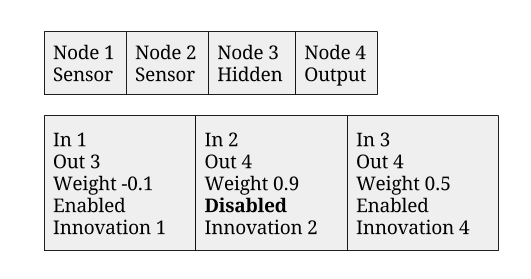
\includegraphics[width=190px]{img/genotype.png}
	\caption[NEAT gene encoding]{An example of a gene encoding of an ANN in NEAT}
	\label{fig:genotype}
\end{figure}

\subsubsection{Speciation}
Speciation in NEAT allows networks with very different topologies to compete, breed and evolve among other networks with largely the same topology.

A new topological innovation in a TWEANN, occurs when a structural change happens, like a new node or a new connection. Such a change is however likely to make the network perform considerably worse than before, compared to the networks in the population, which did not get such a significant change. In order to preserve new innovations, the entire population split into separate species, depending on their topology and they compete, primarily, within their own specie. This way, if a new innovation is placed in a new species, it will be allowed to evolve and tune its new structure to something fitting, and not just be discarded as a bad evolutionary step before it has even been explored.

The following formula is used to calculate the distance between genes for assigning species: 

$$\delta = \frac{c_1E}{N} + \frac{c_2D}{N} + \bar W c_3$$

The formula uses the number of excess genes, $E$, disjoint genes, $D$, and the average weight of the matching genes, $W$. The importance of these three parameters can be adjusted using the three variables $c1$, $c2$ and $c3$, while N is the total amount of genes in the larger of the two networks. There are no definitive optimal settings for these parameters, they have to be experimented with on a case by case basis. The goal of the parameters are to protect innovative changes as they adjust their weights to discover the potential of the change while also discarding structures which have proved not to work. \todo{What is the goal of the adjustment of these hyper parameters? When a innovative change is made, it should be protected}

At each evolution step, a random genome in a species is selected to be that specie's representative, and all other genomes get their distance calculated with regards to that genome, to determine if it should be part of that species. If a genome is too far from any species, then it will be placed in a new species where it, itself will become the representative genome.

All genomes have their fitness changed, depending on how big the species it is part of is, and how different the genomes is from the other genomes in the species:

$$f_i' = \frac{f_i}{\sum^n_{j=1} sh(\delta(i,j))}$$

$f'i$, is the modified fitness of the network, $sh(\delta(i,j))$ is a function returning 1 if $\delta(i,j)$, the distance between the networks, is below the threshold $\delta_t$, otherwise it returns 0. This results in the modified fitness being lower the larger the species the genome is part of is meaning that larger species will have to perform better in order to survive as a large species.

\subsubsection{K-Means speciation} 
\todo{how should this be cited?}http://sharpneat.sourceforge.net/research/speciation-kmeans.html
The framework used for the experiments in this paper does not use the exact speciation strategy described here. It uses K-Means Clustering for speciation which is an algorithm for distributing data points into $K$ different clusters, or in this case, species. The algorithm works by first distributing all genomes into $k$ a random clusters. Then it calculates the centre point for each cluster and continues to distribute all the genomes into the nearest cluster. If a genome has changed cluster during the re-distribution, the algorithm starts again from calculating the centre point of the clusters as they are then and distribute the genomes again. This is done until all clusters are stable or some amount of iterations.

The center point of a cluster is calculated with euclidean distance as the componentwise mean of all the points in a cluster\todo{allowed?}.

K-Means implementation uses a vector of a genes' connection's innovation ids and their weights to represent them in the coordinate system. Manhattan distance is used as the distance metric, which is not much different from the distance metric in the original speciation idea. Manhattan distance in the original distance metric is equal to ${c_1E}$ and ${c_2E}$ set to 0 and $c_3$ to 1.

\subsection{Gradient descent}
Gradient descent is an optimisation method that fits a model to a number of training examples, to learn the underlying data pattern, by minimising a cost function. In the context of image recognition, a training example is an image and associated features, such as the class that the image belongs to. The associated features are referred to as ground truths. The model subject to optimisation is an ANN.

In contrast to NEAT, gradient descent does not adjust the topology of the network. Hence, it is given a predefined topology and thus a set of parameters, known as $\theta$, which is the set of biases of all neurons and weights of all connections in the network. 

Gradient descent iterates through the set of training examples, and calculates cost through backpropagation based on the difference between the predicted features, $a(x)$, and the ground truths, $y(x)$. Euclidean loss is a common cost function.
$$C(x) = {\lVert y(x) - a(x) \rVert}^2$$
The parameters of the network are updated based on the gradient of the cost function $\nabla C$ with respect to $\theta$. By knowing the gradient with respect to every parameter of the network, the parameters can be updated, such that the cost is reduced. Consider a change in cost, as described by the change in a parameter:
$$\Delta C \approx \nabla C \cdot \Delta v $$
If the change in the parameter, $\Delta v$, is chosen, such that $\Delta v = - \eta \nabla C$, where $\eta$ is the learning rate, then it can be shown by substitution that $C$ is reduced.

$$\Delta C \approx - \eta {\nabla C}^2 $$
The learning rate is a small positive number, usually in the range of $10^{-6}$ to $1$. If the learning rate is sufficiently small, then the cost is reduced at every parameter update, but if it set too high, then $\Delta C \approx \nabla C \cdot \Delta v $ is an inaccurate approximation of the change in cost, and the parameter update might result in a rise in cost. \newline

The Euclidean loss cost function presented earlier applied to a single training example. The objective of gradient descent can be described as minimising the average cost for all training examples.

$$C_{Euclidean} = \frac{1}{n} \sum_{x} {\lVert y(x) - a(x) \rVert}^2$$

The true gradient of $C$ is approximated by averaging the gradients calculated from one or more training examples. If parameters are updated from a gradient approximated from one example, the optimisation method is known as stochastic gradient descent. If it is approximated from a number of training examples less than the total number of examples, it is known as mini-batch gradient descent. Mini-batch gradient descent is usually preferred in practice, as it is a good compromise between computational efficiency and accuracy.

\subsubsection{Cost functions}
\label{sec:negative}
For classification tasks, where the output is a probability distribution summing to one, the negative log likelihood is used as cost function. Training examples of classification tasks are represented as a binary vectors, with 1 in the class that the input belongs to. Let $y_{ij}$ be the $j$'th term of the feature vector of the $i$'th training example, and $p_{ij}$ be the corresponding prediction from the network subject to training, then the log likelihood function can be described as:
$$ C_{loglikelihood} = -\frac{1}{n} \sum_{i} \sum_{j} y_{ij}\text{ln}(p_{ij}) $$
Where $n$ is the number of training examples. Explained in more simple terms, the cost of a probability distribution is exactly equal to the negative natural logarithm of the predicted probability of the correct class. Negative log likelihood is preferred over Euclidean loss for classification tasks, as it makes gradient descent converge to the optimal solution faster\cite{Solla}.

The Euclidean loss function described in the last section is used for regression tasks, where any output sum and any output range is allowed.


\subsubsection{Momentum}
Gradient descent, as described above, can be thought of as a ball rolling down a hill until it cannot go any further. However, the speed of the ball is only proportional to the steepness of the curve, and does not accelerate like its physical analogy. While adhering to the laws of physics should not be a motivation in itself, the idea of acceleration in gradient descent has two advantages. It reduces the chance that the ball gets stuck in a local minimum of the cost function, as the momentum of the ball allows it to roll over small hills of the cost function. Secondly, it reduces the number of time steps required to roll down to the bottom of a deep valley. The momentum rules used by Nesterov's Accelerated Gradient (NAG) are slightly different from classical momentum, as it modifies the velocity based on a future position of the ball, rather than the current position. NAG performs an update to the parameters based on the velocity:
$$\theta_{t+1} = \theta_t + v_{t+1}$$
In the non-modified version of gradient descent, the velocity was only based on the gradient. NAG modifies the velocity based on the previous velocity:
$$v_{t+1} = \mu v_t - \eta \Delta C(\theta_t + \mu v_t)$$
Where $\mu$ is a hyperparameter that determines the amount of momentum. It can be shown that NAG converges faster than gradient descent for differentiable and convex cost functions.

\subsubsection{Regularisation}
\label{sec:regularisation}
Regularisation in gradient descent helps preventing the model from overfitting to the training examples. Overfitting occurs, when the optimisation method reduces the models generalisation capabilities, but increases its capabilities of correctly predicting training examples. It occurs as minimising the cost function for the training examples is only an approximate representation of the goal of gradient descent,  the true goal is to make the model generalise. When gradient descent reaches a certain point in training, the only way to get a lower cost is to overfit to the training examples. Early stopping is a strategy to reduce overfitting, by measuring the models generalisation strength on a data set not used during training.

The number of free parameters in a fully connected ANN can be high, as the number of connection weights between to layers are equal to the product of the number of neurons in each layer. A greater number of free parameters increases the overfitting potential of the model, while a greater number of training examples has the opposite effect.
High weights are indicators of overfitting, as an overfitted network detects few unique features of a single example and lets them determine the entire output, to form a "memory" from the parameters. Consequently, both l1- and l2-regularisation limits overfitting by reducing the magnitude of the weights. They do so, by adding a second term to the cost function, such that the change in parameters are influenced by the magnitude of the parameters. Let $C_0$ be the original cost function, then the cost function with l2 regularisation is,
$$C = C_0 + \frac{\lambda}{2n}\sum_{w} w^2 $$
where $\lambda$ is a hyper parameter that dictates the strength of the regularisation. l1 regularisation is very similar, the only difference being that the weights are not squared.

Overfitting can be prevented in other ways. The more training examples gradient descent uses, the less likely overfitting becomes. In the problem domain of this project, training data is readily available, and optimising with additional training data is enough to eliminate overfitting\todo{Ref to results}.

\subsubsection{The vanishing gradient problem}
\label{sec:vanishinggradient}
The vanishing gradient problem is a common problem in deep learning. To understand the solution to the problem, it is necessary to understand some details of the way backpropagation calculates the gradient of the cost function.
Backpropagation works by calculating the error of every neuron, and recursively using the error of the previous neuron to estimate the error of the next error, going backwards. The error of a neuron in the output layer is calculated as: ${\delta}_a = C_a \nabla \cdot f'(z)$. The error of the the neurons in the next layer is based of a product of the derivative of its activation function. The point is, that the further the error travels backwards in the network, the more derivatives gets included in the product. If the derivative is small, the error gets small as well, which leads to small updates to the parameters, which finally leads to slow learning. The sigmoid activation function has an output range of $[0,1]$ and the derivative is calculated as $s'(z) = s(z) \cdot (1-s(z))$. It is apparent that the largest value of $s'(z)$ is $\frac{1}{4}$, and that the derivative gets small in the edges of the range. For examples, in 12 layer network, the error would in the best case scenario be multiplied by ${\frac{1}{4}}^{12} \approx 5.96 \cdot 10^{-8}$. Consequently, this activation function would result in very slow learning in the lower layers. The rectifier activation function partially solves this problem by having a derivative of:
\[
    f'(z) =  
\begin{dcases}
    1,& \text{if } z > 0\\
    0,              & z \leq 0
\end{dcases}
\]
This allows the error to persist through the layers. However, the error is canceled entirely if $z$ is below zero, and the vanishing gradient problem still persists to some degree. If the initialisation of the network results in a ReLU function outputting exclusively zero for all the training examples, it dies and is useless. Consequently, avoiding dying units in the output layer might require multiple initialisations with different seeds. Google's LeNet \cite{christian} additionally addresses the vanishing gradient problem by having multiple output layers calculating outputs from only a subset of the network, thereby reducing the number of steps that the error travels to reach the lowest layers of the network.

\subsubsection{Xavier initialisation}
The initial values of the weights of the network is important when training deep neural networks. Too low weights causes the error signal of backpropagation to stagnate, and too high weights causes the weighted input sum, $z$, to become to large or to small. It is desirable to let be $z$ within a low range, as the non-linearity of the activation function is centered at zero.
Drawing the weights from a normal distribution with a mean of zero and a constant variance does not necessarily keep the weights within the desired range, as the number of inputs varies from neuron to neuron. A neuron with a thousand inputs have a larger variance on its weighted input sum than a neuron with ten inputs, if they both use the same variance.
Xavier et al. \cite{DBLP:journals/jmlr/GlorotB10} suggests an initialisation, where the variance is based on the number of input and output signals, respectively denoted $n_{in}$ and $n_{out}$.
$$ \text{Var}(W) = \frac{2}{n_{in} + n_{out}} $$
This helps keep the weights within a range that makes gradient descent converge faster than with a constant variance.

\subsubsection{Distribution imbalance in classification training data}
\label{sub:data-req}
According to recent research~\cite{balanced-classes} having imbalanced representations of classes used for training with gradient descent can lead to poor performing networks. According to the study, the worst cases of networks trained on imbalanced data were only able to consistently classify images belonging to the most represented class, i.e. one out of a total of ten classes. The imbalance of data were at most a factor of two, i.e the most represented class having twice as many samples as the least represented class.

The complications introduced by imbalanced class distributions can be addressed by evening the distribution of classes. Overcoming the imbalances can be achieved through different approaches.

One method is to delete data from over-represented classes until every class has an equal amount of samples. This can severely affect the amount of training data as data is deleted until every class has samples equal to the lowest denominator.

A second method is proposed in~\cite{balanced-classes}, showing promising results. The idea is to randomly duplicate samples from lesser represented classes, until classes are more evenly distributed. The most extreme form of this method duplicates samples until an even distribution is obtained.
\subsection{Related work}
\label{sec:relatedwork}
In 2014, a visual agent for playing TORCS\footnote{The Open Racing Car Simulator} was developed using reinforcement learning to evolve a network with a CNN component\cite{torcs}. The fitness functions used to train the top layer network was different than the fitness function used to train the CNN component. The top layer network adapted the output of the CNN component and successfully used it, despite the output of the CNN component being humanly incomprehensible, and based solely on the image. The TORCS AI demonstrates the strong input interpretation potential of NEAT.

Chenyi Chen et al. \cite{chen} trained a deep convolutional neural network to detect features of road images in TORCS, retextured to simulate real driving. The features included angle of the road tangent and distance to land markings. The features were translated to driving actions by a handwritten controller, which is the main difference between their and our approach.

The real time shooter Doom has seen several successful AI implementations using convolutional neural networks with reinforcement learning in the Visual Doom AI competition, as for example by Michal Kempka et al.\cite{vizdoom} and Lampre et al.\cite{DBLP:journals/corr/LampleC16}. The domain are similar to ours, but the training methodology differs. Many of the top performing entries for the competition used Deep Q-networks to estimate the Q-value of states. The networks were trained with stochastic gradient descent with data labeled by reinforcement learning. This way of controlling the agent is quite different from out approach, as it is based on a state representation of the game and does not utilize neuroevolution.

Numerous examples of applying supervised learning or evolutionary algorithms to FPS games exist\cite{benjamin}\cite{silvano}, few however uses the visual partially-observable state. This difference is not only significant in terms of the methods required to solve the problem, but also in terms of the expected behaviour of the agent.

\subsection{The FPS setting}
\label{sec:fpssetting}
We obtained the base game and textures used as test bed for our experiments from \url{http://armedunity.com/files/file/107-multiplayer-fps-kit-raknet/} and heavily modified it to suit our needs. This includes removing the ability for bots to shoot and removing everything regarding multiplayer and server functionality. The resulting FPS environment is described in this section.

The agent has a single full automatic weapon, which has 30 bullets in a single magazine. The agent has 6 extra magazines at his disposal. The weapon does not automatically reload when the magazine is empty, in order to force the agent to learn detecting when a magazine is empty. Since the agent does not get any input regarding bullets and magazines left, it should, optimally, learn to count how many bullets and magazines it has used. This is important in order to not waste time attempting to shoot or reload when there are no more bullets or the weapon is fully loaded, it is however possible to get very reasonable behaviour from the agent without perfect reload times.

The target spawns with 100 health points, and a single bullet does 10 damage to it, no matter where it hits. This means that 10 hits are required for the agent to kill the target. If the the agent only reloads when it is out of bullets, it will have 210 bullets, meaning it could theoretically eliminate 21 targets. The agent is however not given enough time to eliminate such a high number of targets, but it is given plentiful extra bullets, to allow for mistakes, in order to increase the learning rate.

The weapon has a violent recoil which the agent has to learn how to control. The recoil is set to miss the enemy/bot already on the third shot in far the most cases and emptying an entire magazine will on average hit the target 3-4 times. As this will result in a very low score, the agent will have to learn how to control the recoil. The recoil is random, so the agent has to learn how to tap-fire in order to maximise accuracy. Had the recoil not been random, as it is seen in games like Counter Strike, then the optimal agent would learn the exact pattern and move and shoot so that all bullets hit the bot as fast as possible. The weapon can shoot 10 times pr. second.

The arena the agent learns in is quadratic, with the agent spawning on one side and the targets spawning on the other, as seen in figure \ref{fig:arena}. Both the agent and the target spawn in a random x and y, while the z coordinate is constant. The first target in the arena always spawn within sight of the agent in order to improve the learning rate. The arena is outfitted with 3 lights to create different visual representations of the target. One light is in the middle of the agent side in order to create differing lightning images of how the agent sees himself. The other two lights are placed on the side of the target, in a way which provide very varied light settings on the target, to test the VRC under different conditions.

\begin{figure}[H]
	\centering
	\begin{scriptsize}
		\sffamily
		\input{img/arena.pdf_tex}
	\end{scriptsize}
	\caption[The FPS game arena]{The arena as seen from above. This illustration omits the y-axis. The lines represent planes, as the agent and the target spawns randomly along both the y-axis and the x-axis.}
	\label{fig:arena}
\end{figure}



















































